
\section{Projection onto the plane of the sky}
\label{sec:projection}

In this section we calculate the apparent shape on the plane of the
sky of the limb-brightened border of a shock or shell that is
idealized as an arbitrary cylindrically symmetric surface.

% Note: I'm aware that some of this material should be moved to an appendix, but I think it will be a future edition.

\subsection{Frames of reference}
\label{sec:ref-frames}

Consider body-frame cartesian coordinates $(x,y,z)$, where \(x\) is
the symmetry axis, and spherical polar coordinates
\((R, \theta, \phi)\), where \(\theta\) is the polar angle and
\(\phi\) the azimuthal angle.  Since the surface is cylindrically
symmetric, it is can be specified as $R = R(\theta)$, so that
cartesian coordinates on the surface are:
\begin{equation}
  \bm{r} \equiv
  \begin{Vector}
    x \\ y \\ z
  \end{Vector} 
  = 
  \begin{Vector}
    R(\theta)\, \cos\theta \\
    R(\theta)\, \sin\theta\cos\phi \\
    R(\theta)\, \sin\theta\sin\phi
  \end{Vector}.
  \label{eq:body-frame}
\end{equation} 
Suppose that the viewing direction makes an angle \(i\) with the
\(z\)~axis, so that we can define observer-frame coordinates
\((x', y', z')\), which are found by rotating the body-frame
coordinates about the \(y\)~axis.  The same vector, \(\bm{r}\), expressed in the observer frame is then 
\begin{equation}
  \bm{r} = 
  \begin{Vector}
    x' \\ y' \\ z'
  \end{Vector}
  = \mathbfss{A}_y(i)\,
  \begin{Vector}
    x \\ y \\ z
  \end{Vector}
  =
  \begin{Vector}
    x\cos i - z\sin i\\
    y \\
    z\cos i + x\sin i
  \end{Vector} \ ,
  \label{eq:Trans}
\end{equation}
where the rotation matrix \(\mathbfss{A}_y(i)\) is given in
Appendix~\ref{sec:plane-sky-projection}.  The inclination angle \(i\)
is defined so that \(i = \ang{0}\) when the surface is viewed
perpendicular to its axis (\textit{side on}) and \(i = \pm\ang{90}\)
when it is viewed along its axis (\textit{end on}), with positive
\(i\) when the apex points towards the observer.


The relationship between the two frames is illustrated in
Figure~\ref{fig:projection-pos}.  All quantities in the observer's
frame are denoted by attaching a prime to the equivalent quantity in
the body frame. There are two ways of interpreting the primed
coordinates. On the one hand, the 3-vector \((x', y', z')\) specifies
a point in Euclidean space, \(\mathds{R}^3\), but an alternative
interpretation is to take the 2-vector \((x', y')\) as specifying a
point in a \textit{projective space}, \(\mathds{P}^2\) (see, for
example, \S~15.6 of \citealp{Penrose:2004a}). Each ``point'' in
\(\mathds{P}^2\) is equivalent to a line in \(\mathds{R}^3\),
specifically: a line of sight that passes through the observer. Thus,
\((x', y')\) gives the celestial coordinates on the \textit{plane of
  the sky}, with \(x'\) being the projected symmetry axis of the
surface.  We assume that the observer is located at a very large
distance, relative to the size of the bow, so that all lines of sight
are effectively parallel to the \(z'\) axis, with the observer at
\(z' = -\infty\).  But, from the point of view of the plane of the sky, the
\(z'\) coordinate is strictly irrelevant since it is a projective
plane, and not a Euclidean plane.  In the following, we will switch
between the \(\mathds{R}^3\) and \(\mathds{P}^2\) interpretations as
convenient, resolving ambiguity where necessary via the adjectives
``Euclidean'' for \(\mathds{R}^3\) and ``plane-of-sky'' or
``projected'' for \(\mathds{P}^2\).



\begin{figure}
  \centering
  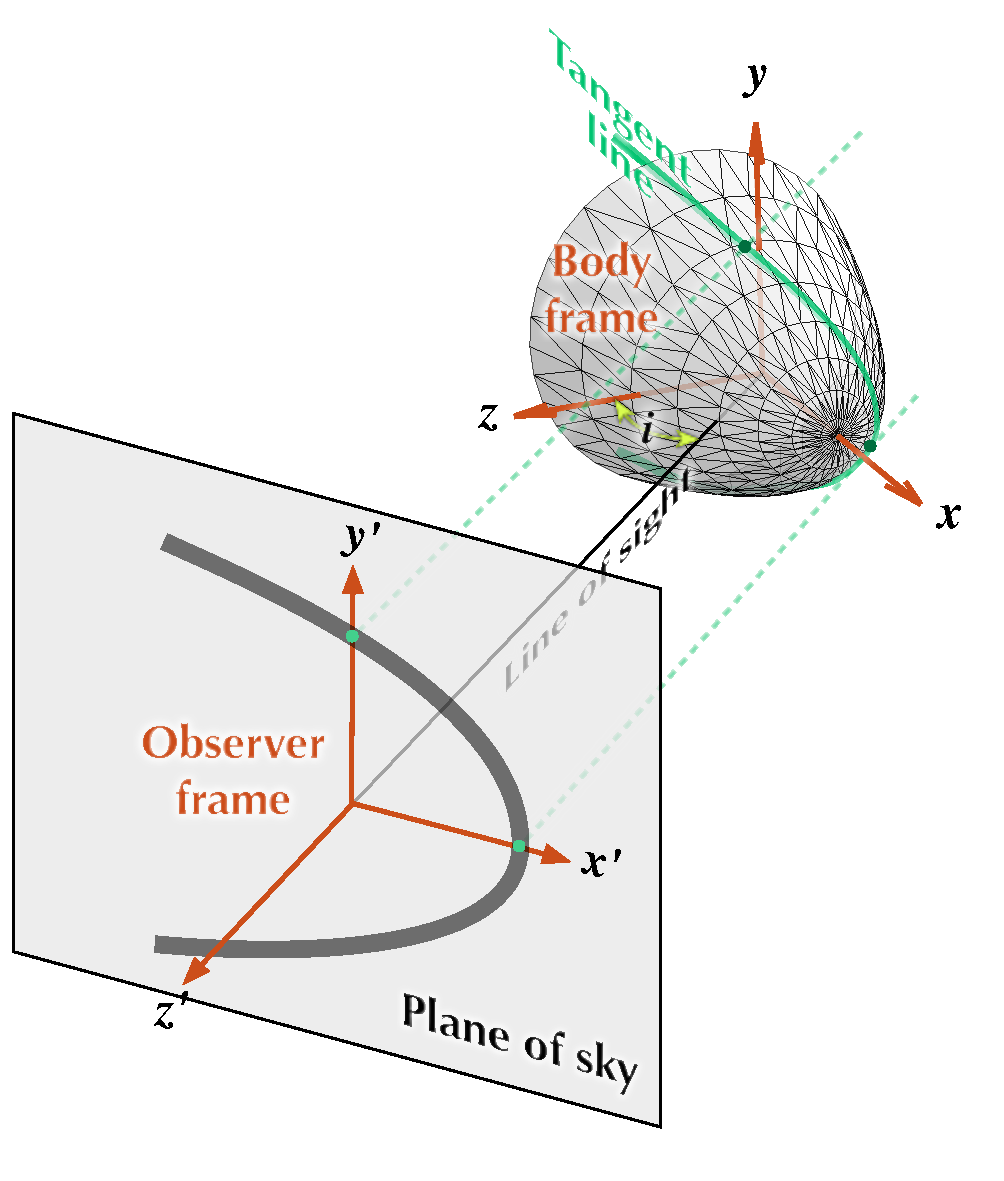
\includegraphics[width=\linewidth]{figs/projection-pos}
  \caption{Relationship between body frame (unprimed coordinates) and
    observer frame (primed coordinates).  Note that the plane of the
    sky is a projective plane, not a geometric plane in Euclidean
    3-space, see discussion in text.}
  \label{fig:projection-pos}
\end{figure}




\subsection{Unit vectors normal and tangential to the surface}
\label{sec:unit-vectors-normal}
\begin{figure}
  \centering
  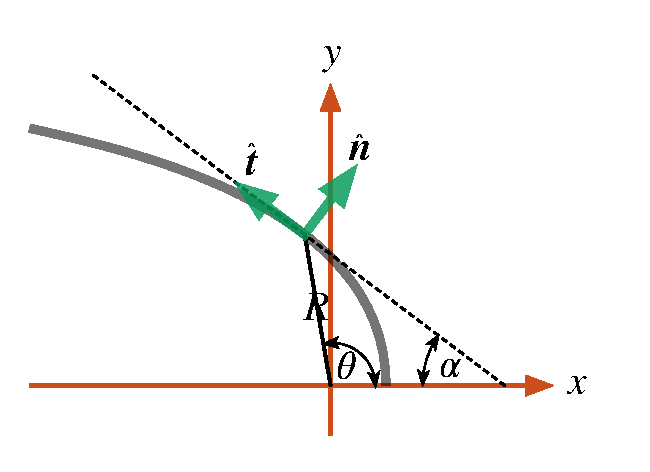
\includegraphics[width=\linewidth]{figs/bowshock-unit-vectors}
  \caption{Unit vectors in the body frame that are normal and
    tangential to the surface \(R(\theta)\) in a plane of constant
    azimuth, \(\phi\).}
  \label{fig:unitvec}
\end{figure}
We define unit vectors \(\uvec{n}, \uvec{t}\), such that \(\uvec{n}\) is normal to the surface, while \(\uvec{t}\) is tangent to the surface in a plane of constant \(\phi\). For \(\phi = 0\) the surface lies in the \(xy\) plane and it is straightforward to show (Fig.~\ref{fig:unitvec}) that in this case the unit vectors are given by 
\begin{equation}
  \label{eq:uvec-phi0}
  \uvec{t}_0 =
  \begin{Vector}
    -\cos\alpha \\ \sin\alpha \\ 0
  \end{Vector}
  \quad \mathrm{and} \quad
  \uvec{n}_0 =
  \begin{Vector}
    \sin\alpha \\ \cos\alpha \\ 0
  \end{Vector}, 
\end{equation}
where \(\alpha\) is the \textit{slope angle}, given by
\begin{equation}
  \label{eq:alpha}
  \tan\alpha = -\left.\frac{dy}{dx}\right\vert_{R(\theta)} 
  = \frac{1 + \omega \tan\theta}{\tan\theta - \omega}
\end{equation}
and \(\omega\) is a dimensionless \textit{local growth factor}:
\begin{equation}
  \label{eq:omega}
  \omega(\theta) = \frac{1}{R} \frac{dR}{d\theta} . 
\end{equation}
For general \(\phi \ne 0\), we find \(\uvec{n}\) and \(\uvec{t}\) by
rotating equations~(\ref{eq:uvec-phi0}) around the \(x\)-axis with the
matrix \(\mathbfss{A}_x(\phi)\) (eq.~[\ref{eq:Rotation-matrix-x}]):
\begin{align}
  \label{eq:uvec-n-phi}
  \uvec{n} &= \mathbfss{A}_x(\phi) \, \uvec{n}_0 =
  \begin{Vector}
    \sin\alpha \\ \cos\alpha\cos\phi \\ \cos\alpha\sin\phi
  \end{Vector}  \\
  \label{eq:uvec-t-phi}
  \uvec{t} &= \mathbfss{A}_x(\phi) \, \uvec{t}_0 =
  \begin{Vector}
    -\cos\alpha \\ \sin\alpha\cos\phi \\ \sin\alpha\sin\phi
  \end{Vector} \ .
\end{align}

\subsection{Tangent line}
\label{sec:tangent-line}

% For optically thin emission with isotropic emissivity \(j\), the observed
% surface brightness for any line of sight that intersects the shell is
% \(S = \int j \, dz' / 4\pi\). 
 
% If the shell thickness is \(h(\theta)\) and emissivity is
% \(j(\theta)\), then for optically thin emission the observed
% surface brightness for any line of sight that intersects the shell is
% \(S = j s / 4\pi\), where \(s\)

% in the limit \(h \ll R\) and
% \(\mu\) is
% the cosine of the angle between the line of sight and the local normal
% to the shell surface at the point of intersection:
% \begin{equation}
%   \label{eq:2}
%   \mu = \uvec{n} \cdot \uvec{z}'
% \end{equation}

The boundary on the plane of the sky of the projected surface is the
locus of those lines of sight that graze the surface tangentially.
This corresponds to a curved line on the surface itself, which we
denote the \textit{tangent line}, and which is defined by the
condition  
\begin{equation}
  \label{eq:tangent-line-condition}
  \uvec{n} \cdot \uvec{z}' = 0.
\end{equation}
We denote by \(\phi\T\) that value of $\phi$ that satisfies this relation
for a given inclination, \(i\), and polar angle, \(\theta\).  From
equations~(\ref{eq:uvec-n-phi}, \ref{eq:tangent-line-condition},
\ref{eq:zunit-prime}, \ref{eq:alpha}) this is
\begin{equation}
\sin\phi\T = -\tan i\tan\alpha = \tan i \frac{1+\omega\tan\theta}{\omega-\tan\theta} \ .
\label{eq:tanphi}
\end{equation}
From equations~(\ref{eq:body-frame}, \ref{eq:Trans}) it follows that
the observer-frame coordinates of the tangent line are given by
\begin{equation}
\left(\begin{array}{c}
x'\T \\ y'\T \\ z'\T
\end{array}\right)= R(\theta)\left(\begin{array}{c}
\cos\theta\cos i - \sin\theta\sin\phi\T \sin i \\
\sin\theta(1-\sin^2\phi\T)^{1/2} \\
\cos\theta\sin i +\sin\theta\sin\phi\T\cos i
\end{array}\right).
\label{eq:tangential}
\end{equation} 
Note that, in general, \(z'\T\) is not a linear function of \(x'\T\)
and \(y'\T\), so that the tangent line \((x'\T, y'\T, z'\T)\) is not a
plane curve in 3-dimensional Euclidean space, \(\mathds{R}^3\).
However, for the projected shape \((x'\T, y'\T)\) of the tangent line
on the plane of the sky, \(\mathds{P}^2\), the value of \(z'\T\) does
not matter (see above).  The projected shape can also be described in
polar form as \(R'(\theta')\), where
\begin{equation}
  \label{eq:R-prime-theta-prime}
  R' = (x'^2\T+ y'^2\T)^{1/2} 
  \quad \text{and} \quad
  \tan\theta' = y'\T / x'\T.
\end{equation}

Equation~(\ref{eq:tanphi}) will not have a solution for
arbitrary values of $\theta$ and $i$, but only when
$|\tan i\tan\alpha|<1$. In particular, if $i\neq 0$, then the tangent line
only exists for \(\theta > \theta_{0}\) where \(\theta_{0}\) is the value of
\(\theta\) on the tangent line's projected symmetry axis
(\(\theta' = 0\)).  From equations~(\ref{eq:tangential},
\ref{eq:R-prime-theta-prime}) it follows that \(\sin^2\phi\T = 1\) at
\(\theta = \theta_0\), which yields the implicit equation
\begin{align}
\tan\theta_{0} = \frac{|\tan i| + \omega(\theta_{0})}{1-\omega(\theta_{0}) |\tan i|} . 
\label{eq:thetapar}
\end{align}
In addition, if the surface is sufficiently ``open''
(\(\alpha \ge \alpha_{\mathrm{min}} > 0\) for all \(\theta\)), then for those
inclinations with
\(\vert i\vert > (\ang{90} - \alpha_{\mathrm{min}}) \) the tangent line does not exist
for any value of \(\theta\).  In other words, when the viewing angle is
sufficiently close to face-on, the projected surface has no ``edge''
and will no longer look like a bow shock to the observer.

After completing this work, it was brought to our attention that the
principal results of this section had already been derived in
Appendix~B of the PhD thesis \citet{Wilkin:1997a}.  For instance,
Wilkin's equation~(8) is equivalent (apart from differences in
notation) to our equation~\eqref{eq:tanphi}.

\subsection{Characteristic radii on the plane of the sky}

% Considering further applications to bow shocks, we will consider open shells.
In order to compare the shell shape given by $R(\theta)$ with observations,
it is convenient to define the following apparent radii in the
observer frame: $R'_{0}$ and $R'_{90}$. These are projected distances
of the shell tangent line from the origin. The first is measured in
the direction of the symmetry axis, and the second in a perpendicular
direction. More concretely $R'_{0} = x'\T(y'\T=0)$ and
$R'_{90} = y'\T(x'\T=0)$. From equations (\ref{eq:tanphi}) and
(\ref{eq:tangential}) we find that:
\begin{align}
R'_{0} = R(\theta_{0})\cos(\theta_{0} + i) \label{eq:Rpar} 
\end{align}
Where $\theta_{0}$ is the solution of equation (\ref{eq:thetapar}), and
\begin{align}
  \label{eq:R90prime}
R'_{90} = R(\theta_{90})\sin\theta_{90}\left(1-\sin^2\bigl(\phi\T(\theta_{90})\bigr)\right)^{1/2}
\end{align}
Where $\theta_{90}$ is the solution of the implicit equation:
\begin{align}
  \label{eq:th90}
\cot\theta_{90} = \frac{1-\left(1+\omega(\theta_{90})^2\sin^22i\right)^{1/2}}{2\omega(\theta_{90})\cos^2 i}
\end{align}
The projected alatude (see \S~\ref{sec:plan-alat-bow}) is then given
by \(\Lambda' = R_{90}' / R_0'\).

Similarly, the projected planitude is \(\Pi' = R_{\C}' / R_0'\), where
\(R_{\C}'\) is found by applying the equivalent of equation
\eqref{eq:radius-curvature} for primed quantities:
\begin{equation}
  \label{eq:projected-radius-curvature}
  R_{\C}' 
  = \frac{(R_0')^2}{R_0' - R_{\theta'\theta',0}'} \ .
\end{equation}


\subsection{Line-of-sight velocities on the tangent line}
\label{sec:line-sight-veloc}
Motions in a thin shocked shell will be predominantly tangential to
the shell surface. In addition, for the particular case of wind-wind
bowshocks, the flow in each azimuthal slice can be shown to be
independent \citep{Wilkin:2000a}, which implies that the shell
velocity is parallel to \(\uvec{t}\). The projected line-of-sight
shell velocity is therefore
  \begin{equation}
    \label{eq:vlos}
    v_{\mathrm{los}} = (\uvec{t}' \cdot -\uvec{z}') \, v_{\parallel}(\theta) = \frac{v_{\parallel}(\theta) (1+\omega^2)^{1/2} \sin i }{\sin\theta - \omega\cos\theta} ,
  \end{equation}
  where \( v_{\parallel}(\theta)\) is the gas velocity along the shell and the standard sign convention has been adopted such that velocities away from the observer are deemed positive. 


%%% Local Variables:
%%% mode: latex
%%% TeX-master: "quadrics-bowshock"
%%% End:

